\documentclass[12pt]{article}

% Include Theme
% Margins ----------------------------------------------------------------------

\usepackage[margin=1.25in]{geometry}

% AMS --------------------------------------------------------------------------

\usepackage{amsmath}
\usepackage{amsfonts}
\usepackage{amsthm}
\usepackage{graphicx}


% Line Spacing -----------------------------------------------------------------

\renewcommand{\baselinestretch}{1.5}


% Font -------------------------------------------------------------------------

\usepackage[T1]{fontenc}
\usepackage[default]{lato}
% \usepackage[utopia, varg]{newtxmath}
% \renewcommand{\rmdefault}{futs} % Utopia as text font 

% Small adjustments to text kerning
\usepackage{microtype}

% Remove annoying over-full box warnings
\vfuzz2pt 
\hfuzz2pt


% Tikz support -----------------------------------------------------------------

\usepackage{tikz}


% Color Palette ----------------------------------------------------------------

\usepackage{xcolor}

% https://www.materialpalette.com/colors
\definecolor{dark-maroon}{HTML}{5D0F0D}
\definecolor{navyblue}{HTML}{0A3044}

% https://www.viget.com/articles/color-contrast/
\definecolor{purple}{HTML}{5601A4}
\definecolor{navy}{HTML}{0D3D56}
\definecolor{ruby}{HTML}{9a2515}
\definecolor{alice}{HTML}{107895}
\definecolor{daisy}{HTML}{EBC944}
\definecolor{coral}{HTML}{F26D21}
\definecolor{kelly}{HTML}{829356}
\definecolor{cranberry}{HTML}{E64173}
\definecolor{jet}{HTML}{131516}
\definecolor{asher}{HTML}{555F61}
\definecolor{slate}{HTML}{314F4F}


% Hyperlinks -------------------------------------------------------------------

\usepackage{hyperref}
\hypersetup{
    colorlinks= true,
    citecolor= dark-maroon,
    linkcolor= dark-maroon,
    filecolor= dark-maroon,      
    urlcolor= dark-maroon,
}


% Citations --------------------------------------------------------------------

% note, natbib provides better hyperlinking
\usepackage{natbib}
\bibliographystyle{econ-aea}
% How to display multiple in \citet{}
\setcitestyle{comma,aysep={}}

% Define Theorems --------------------------------------------------------------

% Put proper spacing after Theorem #. 
\newtheoremstyle{spacing}
{}%          Space above, empty = `usual value'
{}%          Space below
% {\itshape}%  Body font
{}%  Body font
{}%          Indent amount (empty = no indent, \parindent = para indent)
{\bfseries\color{navyblue}}% Thm head font
{.\ }%         Punctuation after thm head
{2.5mm}%  Space after thm head: \newline = linebreak
{}%          Thm head spec

% note, theorem is the name that goes in \begin{} and Theorem is the name displayed as Theorem 1
\theoremstyle{spacing}
\newtheorem{theorem}{Theorem}
\newtheorem{proposition}{Proposition}
\newtheorem{assumption}{Assumption}
\newtheorem{remark}{Remark}
\newtheorem{example}{Example}


% Custom Math Definitions ------------------------------------------------------

\global\long\def\expec#1{\mathbb{E}\left[#1\right]}%
\newcommand{\condexpec}[2]{\mathbb{E}\left[#1 \ \vert \ #2\right]}
\global\long\def\prob#1{\mathbb{P}\left[#1\right]}%
\global\long\def\var#1{\mathrm{Var}\left[#1\right]}%
\global\long\def\cov#1{\mathrm{Cov}\left[#1\right]}%
\global\long\def\one{\mathbf{1}}%


% Titlepage --------------------------------------------------------------------

% \maketitle
\usepackage{titling}
\usepackage{setspace}

% title
\pretitle{\begin{spacing}{1}\begin{flushleft}\huge}
\posttitle{\end{flushleft}\end{spacing}\vspace{-5mm}}
% author, note don't use \and 
\preauthor{\begin{flushleft}\LARGE}
\postauthor{\end{flushleft}\vspace{-7.5mm}}
% date
\predate{\begin{flushleft}\Large\color{asher}}
\postdate{\end{flushleft}\vspace{-5mm}}

% Abstract
\renewenvironment{abstract}
 {\noindent\rule{\linewidth}{.5pt}\noindent}
 {\noindent\rule{\linewidth}{.5pt}}

% alternative abstract
% \renewenvironment{abstract}
% {
%   \centerline {\large \bfseries \scshape \color{navyblue} Abstract}
%   \begin{quote}
% }
% {\end{quote}}


% Section and Subsection Styling -----------------------------------------------

\usepackage[explicit]{titlesec}

\titleformat{\section}
  {\large \bf \color{navyblue}}
  {\thesection \,---}
  {0.25em}
  {#1}
  
\titleformat{\subsection}
  {\fontsize{11}{10}\it}
  {\thesubsection.}
  {1em}
  {#1}


% Footnote ---------------------------------------------------------------------

% Spacing between footnotes on same page
\addtolength{\footnotesep}{1mm}

% Space after footnote number
\let\oldfootnote\footnote
\renewcommand\footnote[1]{\oldfootnote{\ #1}}

% No footnote line
\renewcommand\footnoterule{}

% No supsercript in footer
\makeatletter
\renewcommand\@makefntext[1]{%
    \parindent 1em \noindent
    \hb@xt@1.8em{\hss\normalfont\@thefnmark.\hfill}#1
  }
\makeatother




% Enumerate/Itemize ------------------------------------------------------------

\usepackage{enumitem}
\setitemize{labelindent=0.5em,labelsep=0.25cm,leftmargin=*}
\setenumerate{labelindent=0.5em,labelsep=0.25cm,leftmargin=*}


% Table and Figure labelling ---------------------------------------------------

\usepackage{caption}

\DeclareCaptionLabelSeparator{threedash}{\,---\,}
\DeclareCaptionFont{navyblue}{\color{navyblue}}
\DeclareCaptionFont{jet}{\color{jet}}
\captionsetup[table]{format=plain, labelsep=threedash, font={navyblue, bf}}
\captionsetup[figure]{format=plain, labelsep=threedash, font={navyblue, bf}}

% Alternative: Left align captions
% \captionsetup[table]{labelfont=it, textfont={navyblue, bf}, labelsep=newline, justification=raggedright, singlelinecheck=off}
% \captionsetup[figure]{labelfont=it, textfont={navyblue, bf}, labelsep=newline, justification=raggedright, singlelinecheck=off}

% multifigure with \caption
% \begin{subfigure}\caption{} \end{subfigure}
\usepackage{subcaption}
\captionsetup[subfigure]{format=plain, font={jet, footnotesize, bf}}


% Tables -----------------------------------------------------------------------

% Fix \input with tables
% \input fails when \\ is at end of external .tex file
\makeatletter
\let\input\@@input
\makeatother

% Make tables/figures wider than \textwidth using:
% \begin{adjustbox}{width = 1.2\textwidth, center}
% \end{adjustbox}
\usepackage{adjustbox}

% Slighty more spacing between rows
\usepackage{array}
\renewcommand\arraystretch{1.25}

% Table with easy to use footnotes
% \begin{threeparttable}
%    \begin{tabular} ... \end{tabular}
%    \begin{tablenotes}
%        \item \textit{Notes.}
%    \end{tablenotes}  
% \end{threeparttable}
\usepackage[flushleft]{threeparttable}
\setlength\labelsep{0pt}

% \toprule, \cmidrule, \bottomrule
\usepackage{booktabs}

% If tables are too narrow, fill columns using:
% \begin{tabularx}{\linewidth}{cols}
% col-types: X - center, L - left, R -right
% If you want relative scale for columns: 
% >{\hsize=.8\hsize}X/L/R
\usepackage{tabularx}
\newcolumntype{L}{>{\raggedright\arraybackslash}X}
\newcolumntype{R}{>{\raggedleft\arraybackslash}X}
\newcolumntype{C}{>{\centering\arraybackslash}X}

% Landscape table 
% \begin{landscape} \pagestyle{lscaped} table... \end{landscsape}
% \usepackage{pdflscape} - rotates page left-side up in pdf
% \usepackage{lscape} - does not rotate page, only figure/table

\usepackage{pdflscape}

% For landscape, fix page number location
\usepackage{fancyhdr}
\fancypagestyle{lscaped}{%
    \fancyhf{}
    \renewcommand{\headrulewidth}{0pt}
    \textnormal
    \fancyfoot{%
        \tikz[remember picture,overlay]
        \node[outer sep=2.5cm,above,rotate=90] at (current page.east) {\thepage};
    }
}
  

% ------------------------------------------------------------------------------


% \maketitle info
\title{Difference-in-Differences with Geocoded Microdata\thanks{I am grateful to Max Farrell, Taylor Jaworski, Damian Clarke, Alexander Bentz, James Flynn, Brach Champion, and Hannah Denker for the helpful insights.}}
\author{\href{https://kylebutts.com/}{Kyle Butts}\thanks{University of Colorado, Boulder. Corresponding Author. Email: \href{mailto:kyle.butts@colorado.edu}{kyle.butts@colorado.edu}.} % \ and Other Author}
}
\date{\today}

\newcommand{\dist}{\text{Dist}}

% pdf info
\hypersetup{pdftitle={Difference-in-Differences with Geocoded Microdata}, pdfauthor={Kyle Butts}}

\begin{document}

% Title Page -------------------------------------------------------------------
\begin{titlepage}
\maketitle

\begin{abstract}
    I formalize a commonly-used estimator for the effects of spatially-targeted treatment with geocoded microdata. This estimator compares units immediately next to treatment to units slightly further away. I introduce intuitive identifying assumptions for the average treatment effect among affected units and illustrate problems when these assumptions fail. Since one of these assumptions requires knowledge of exactly how far treatment effects are experienced, I propose a new method that allows for nonparametric estimation following methods introduced in \citet{Cattaneo_Farrell_Feng_2019}. Since treatment effects can change with distance, the proposed estimator improves estimation by estimating a \emph{treatment effect curve}.

    \par~\par\noindent
    {\color{asher}JEL-Classification:} C13, C14, C18
    \par\noindent
    {\color{asher}Keywords:} Spatial Econometrics, Spillover Effects, Difference-in-Differences, Nonparametric Estimation
    \par\vspace{-2.5mm}
\end{abstract}
\end{titlepage}

% Paper ------------------------------------------------------------------------

% ------------------------------------------------------------------------------
\section{Introduction}
% ------------------------------------------------------------------------------

The rise of geocoded microdata has allowed researchers to begin answering questions about the effects of spatially-targeted treatments at a very granular level. How do local pollutants affect child health?\footnote{See, e.g., \citet{Currie_Davis_Greenstone_Walker_2015} and \citet{Marcus_2021}.} Does living within walking distance to a new bus stop improve labor market outcomes?\footnote{See, e.g., \citet{Gibbons_Machin_2005} and \citet{Billings_2011}.} How far do neighborhood shocks, such as foreclosures or new construction spread?\footnote{See, e.g., \citet{Asquith_Mast_Reed_2021,Cui_Walsh_2015,Gerardi_Rosenblatt_Willen_Yao_2015} and \citet{Campbell_Giglio_Pathak_2011}.} A standard method of evaluating the effects of the treatment is to compare changes in outcomes for units that are close to treatment to those slightly further away -- what I label the `ring method' as illustrated in \autoref{fig:example-id}. This paper formalizes the assumptions required for identification in the ring method, highlighting potential pitfalls of the currently-used estimator, and proposes an improved estimator. 

First, I formalize the necessary assumptions for unbiased estimates of the average treatment effect on the affected units.\footnote{This generalizes the treatment effect on the treated in the case where treatment is not assigned to specific units.} The first assumption is the well understood parallel trends assumption for the treated and control units. This requires that the \emph{average} change in (counterfactual) untreated outcomes in the treated ring is equal to the \emph{average} change in the control ring. The rings method is typically motivated by the fact that since the treated and control units are all very close in physical location, e.g. having access to the same labor market and consumptive amenities, shocks over time should be common across units in the neighborhood.\footnote{For example, \citet{Asquith_Mast_Reed_2021} write "The idea is that within a small area, developers have few sites that are available and properly zoned, leading to hyper-local variation in the location of new construction that is not related to future price changes."} 

Instead of \emph{fully} leveraging the common neighborhood trends assumption that motivates the ring method, researchers rely on a second assumption which requires correct identification of how far treatment effects are experienced (the inner ring). This is a very strict assumption that when not satisfied, causes biased estimates of the treatment effect. If the treated ring is too narrow, then units in the control ring experience effects of treatment and the change among `control' units would no longer identify the counterfactual trend. On the other hand, if the treated ring is too wide, then the zero treatment effect of some unaffected units are averaged into the change among `treated' units. Therefore, results will be attenuated towards zero.

% Figure: Example ID -----------------------------------------------------------

\begin{figure}[tb]
  \caption{Rings Method}
  \label{fig:example-id}

  \begin{adjustbox}{width = 0.4\textwidth, center}
      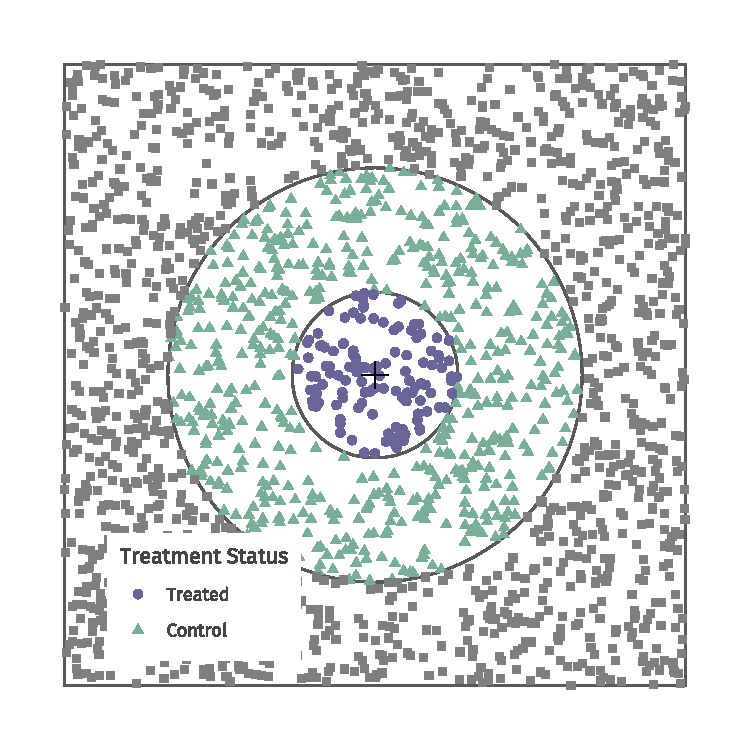
\includegraphics[width=\textwidth]{../../figures/example_id.pdf}
  \end{adjustbox}

  {\footnotesize
    \emph{Notes:} This figure illustrates the ring method. The center triangle represents the location of treatment, e.g. a foreclosed home. Units within the inner circle, marked by dots, are considered `treated'; units between the inner and outer circles, marked in triangles, are considered control units; and then the remaining units are removed from the sample. The ring estimate compares average changes in outcomes between the inner `treated' ring and the outer `control' ring.
  }
\end{figure}

I propose an alternative estimator that fully leverages the `common neighborhood trends' assumption using a nonparametric partitioning-based least square estimator \citep{Cattaneo_Crump_Farrell_Feng_2019,Cattaneo_Farrell_Feng_2019}. My proposed methodology estimates the treatment effect curve as a function of distance by using many rings rather than trying to estimate the average treatment effect with one inner ring. This method requires that treatment effects become zero somewhere between the distance of 0 and the outer ring \emph{without} the need to specify the \emph{exact} distance at which it does. To do this, the estimator leverages the stronger `common neighborhood trends' assumption that the counterfactual trend is constant across distance. This new assumption is more strict in that the standard method only requires that parallel trends holds \emph{on average} in each ring. However, researchers typically motivate the identification strategy by saying within a small distance from treatment that units are subject to a common set of shocks which implies the more strict assumption. While this assumption is not directly testable, my proposed estimator creates a set of point estimates of treatment effects that can be used to visually inspect the plausability of the assumption. If after some distance, treatment effects become centered at zero, this suggests that common trends hold, akin to the pre-trends test in event study regressions.

The nonparametric estimator provides many benefits. First, the estimator allows the researcher to get a more complete picture of how the intervention affects units at various distances rather than estimating an ``overall effect''. For example, a new bus-stop potentially creates net costs to immediate neighbors while providing net benefits for homes slightly further away. Estimation of the treatment effect curve can illustrate these different effects that a single ring may average out to near-zero effects. Additionally, the proposed nonparametric estimator selects the rings in a \emph{completely data-driven and optimal manner} removing incentives for specification searching or `pre-testing' the data to determine the `correct' rings \citep{McCloskey_Michaillat,Andrews_Kasy}.

This paper contributes to the literature in many ways. First, I contribute to a literature that discuss identification using the rings method. \citet{Sullivan_2017} and \citet{Gerardi_Rosenblatt_Willen_Yao_2015} discuss the identification assumption of identifying the maximum treatment distance. My paper formalizes all the necessary assumptions for identification in the ring method. Other researchers have recognized that estimating a single average treatment effect is less informative than a treatment effect curve, instead using multiple rings to estimate treatment effects at different distances (e.g. \citet{Alexander_Currie_Schnell_2019,Casey_Schiman_Wachala_2018,Di_Tella_Schargrodsky_2004}). However, this approach selects multiple rings in an ad-hoc manner, requires treatment effects to become zero after the outer-most treatment ring, and is prone to problems of specification searching. The current study's proposed estimator selects the number and location of rings in a data-driven way and does not require correct specification of where treatment effects become zero.

\citet{Diamond_McQuade_2019} propose an alternative nonparametric estimator aimed at estimating a treatment effect surface. Similar to this paper, they leverage the "common local trends" assumption to estimate a \emph{two-dimensional} treatment effect curve. Their procedure allows ``location'' fixed effects to differ along two-dimensions, latitude and longitude (e.g. the mean home price is higher in the north-west than the south-east) which in cross-sectional data can absorb more variation in the data yielding smaller standard errors than my method, though both are consistent. In the case of panel data, this does not matter since first-differencing remove this systematic variation. To produce noise estimates/standard errors, their method requires integrating over the 2D curve for arbitrarily chosen rings. In cases where researchers chose these aggregation ranges based on the results of the estimation procedure, standard inference tools are not valid even when bootstrapping the standard errors \citep{Leeb_Potscher_2005}. As discussed above, my proposed estimator provides valid inference after selection of aggregation regions and choses these aggregation regions in a data-driven manner.

This paper also contributes to a small literature on difference-in-differences estimators from a spatial lens \citep{Butts_2021,Clarke_2017,Berg_Streitz_2019,Verbitsky-Savitz_Raudenbush_2012,Delgado_Florax_2015}. These papers address instances where treatment is well defined by administrative boundaries but spillovers cause problems of defining who is `treated' and at what level of exposure. This paper contributes to this literature by considering the setting where treatment occurs at a point in space. \citet{Butts_2021} and \citet{Clarke_2017} both recommend a method of using many rings to estimate a treatment effect curve, but are not able to provide a data-driven way to select the rings. Since this paper focuses on local shocks where constant parallel trends are plausible, I am able to provide a data-driven approach to choosing rings. 

% ------------------------------------------------------------------------------
\section{Example of Problem}\label{sec:example}
% ------------------------------------------------------------------------------

% Figure: Example problem ------------------------------------------------------

\begin{figure}[tb]
  \caption{Example of Problems with Ad-Hoc Ring Selection}
  \label{fig:problems}

  \begin{adjustbox}{width = 1.1\textwidth, center}
      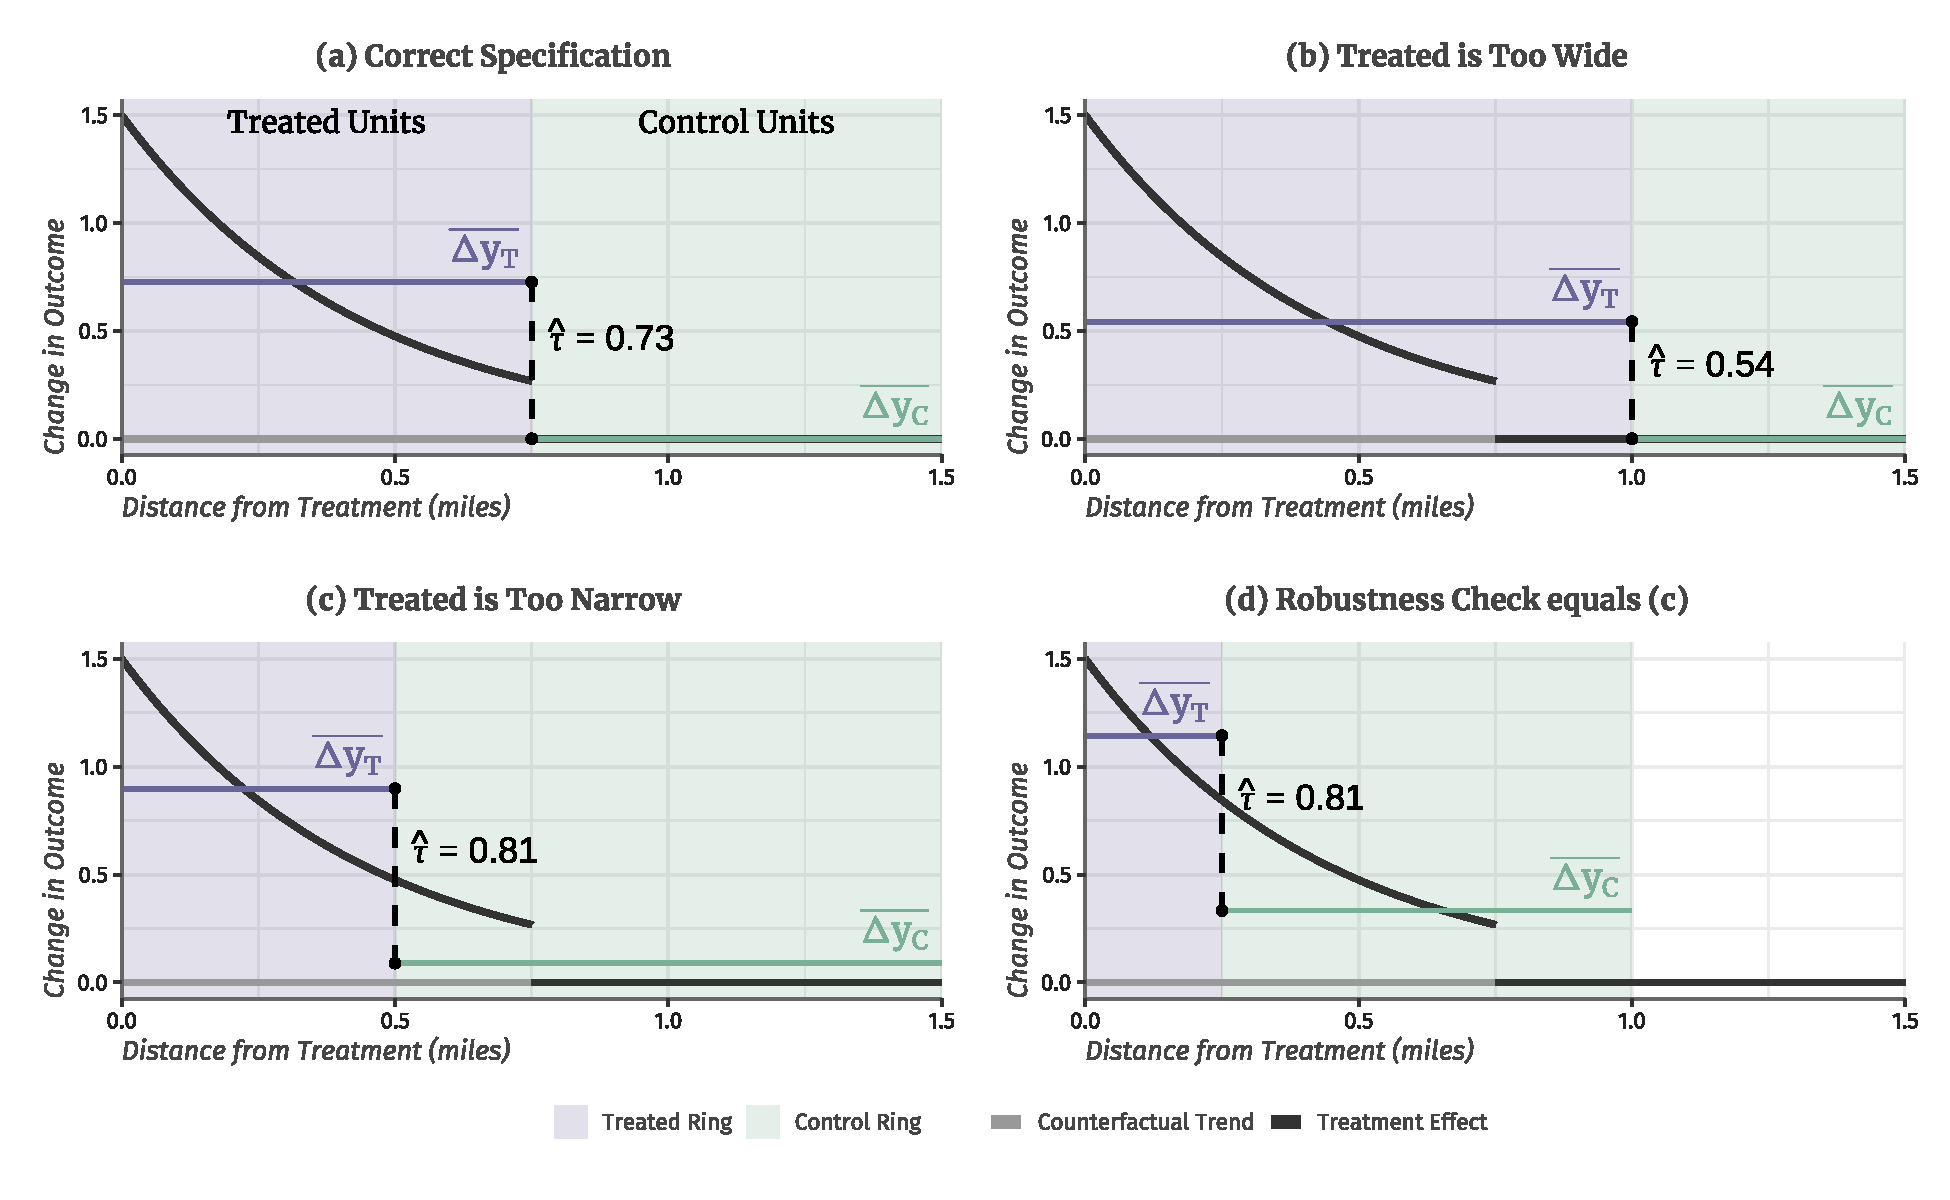
\includegraphics[width=\textwidth]{../../figures/example.pdf}
  \end{adjustbox}

  {\footnotesize \emph{Notes:} This figure shows an example of the difficulties in estimation of treatment effects via the ring method.}
\end{figure}

To illustrate the methodological difficulties in this method, suppose that an overgrown empty lot in a high-poverty neighborhood is cleaned up by the city and the outcome of interest is home prices. The researcher observes a panel of home sales before and after the lot is cleaned. \autoref{fig:problems} shows a plot of simulated data from this example. The black line is treatment effect at different distances from the empty lot and the grey line is the underlying (\emph{constant}) counterfactual change in home prices, normalized to 0. Panel (a) of \autoref{fig:problems} shows the best-case scenario where the treated ring is correctly specified. The two horizontal lines show the average change in outcome in the treated ring and the control ring and our treatment effect estimate, $\hat{\tau}$, is the difference between these two averages. However, this singular number masks over a large amount of treatment effect heterogeneity with units experiencing treatment effects as little as half and as large as double the magnitude that of $\hat{\tau}$. Later in this paper, I recommend nonparametrically estimating the treatment effect curve as a function of distance rather than using average effect. 

However, the researcher does not typically know the distance at which treatment effects stop. Panel (b) shows when the `treatment' ring is too wide. In this case, some of the units in the treatment ring receive no effect from treatment and therefore makes the average treament effect among units in the treatment ring smaller. Panel (c) of \autoref{fig:problems} shows the opposite case, where the treated ring is too narrow. In this case, there are some units in the `control' ring that experience treatment effects and the coutnerfactual trend estimate is biased upward. The treatment effect estimate grows since the new `treated' group is closer and hence experiences larger treatment effects. Panel (d) of \autoref{fig:problems} shows an example of why using different rings as a `robustness check' is a problematic practice. Using Panel (d) as a robustness check for the researchers' original specification of Panel (c), a researcher would be quite confident in their results even though the estimate is too large in both cases.

From these three examples, it's clear that the estimation strategy requires researchers to know the exact distance at which treatment effects become zero. Since this is a very demanding assumption, I propose an improved estimator in \autoref{sec:lspartition} that relaxes this assumption by leveraging the constant common trends assumption. 




% ------------------------------------------------------------------------------
\section{Theory}
% ------------------------------------------------------------------------------

Now, I develop econometric theory to formalize the intuition developed in the previous section. A researcher observes panel data of a random sample of units $i$ at times $t = 0, 1$ located in space at point $\theta_i = (x_i, y_i)$. Treatment occurs at a location $\bar{\theta} = (\bar{x}, \bar{y})$ between periods. Therefore, units differ in their distance to treatment, defined by $\dist_i \equiv d(\theta_i, \bar{\theta})$ for some distance metric $d$ (e.g. Euclidean distance) with a distribution function $F$. Outcomes are given by 
\begin{equation}
    Y_{it} = \mu_i + \tau_i \one_{t = 1} + \lambda_i \one_{t=1} +u_{it},    
\end{equation}
where $\mu_i$ is unit-specific time-invariant factors, $\lambda_i$ is the change in outcomes due to non-treatment shocks in period 1, $\tau_i$ is unit $i$'s treatment effect. Both $\lambda$ and $\tau$ can be split into a systematic function of distance $z(\dist_i)$ and an idiosyncratic term $\tilde{z}_i \equiv z_i - z(\dist_i)$ with $z$ being $\tau$ and $\lambda$. $\tau(d)$ is the average effect of treatment at a given distance and $\lambda(d)$ summarizes how covariates and shocks change over distance.

Therefore, we could rewrite our model as 
\begin{equation}\label{eq:model}
    Y_{it} = \mu_i + \tau(\dist_i) \one_{t = 1} + \lambda(\dist_i) \one_{t=1} + \varepsilon_{it},   
\end{equation}
where $\varepsilon = u_{it} + \tilde{\tau}_i + \tilde{\lambda}_i$ which is uncorrelated with distance to treatment. Researchers are trying to identify the average treatment effect on units experiencing treatment effects, i.e. $\bar{\tau} = \condexpec{\tau_i}{\tau(\dist_i) > 0}$.

\begin{assumption}[Random Sampling]
    The observed data consists of $\{ Y_{i1}, Y_{i0}, \dist_{i}\}$ which is independent and identically distributed.
\end{assumption}

Taking first-differences of our model, we have $\Delta Y_{it} = \tau(\dist_i) + \lambda(\dist_i) + \Delta \varepsilon_{it}$. It is clear that $\tau(\dist_i)$ and $\lambda(\dist_i)$ are not seperately identified unless additional assumptions are imposed. The central identifying assumption that researchers claim when using the ring method is that counterfactual trends likely evolve smoothly over distance, so that $\lambda(\dist_i)$ is approximately constant within a small distance from treatment. This is formalized in the context of our outcome model by the following assumption. 

\begin{assumption}[Local Parallel Trends]\label{assum:parallel}
    For a distance $\bar{d}$, we say that `local parallel trends' hold if for all positive $d, d' \leq \bar{d}$, then $\lambda(d) = \lambda(d')$.
\end{assumption}

This assumption requires that, in the absence of treatment, outcomes would evolve the same at every distance from treatment within a certain maximum distance, $\bar{d}$. To clarify the assumption, it is helpful to think of ways that it can fail. First, if treatment location is targeted based on trends \emph{within a small-area/neighborhood}, then trends would not be constant within the control ring. Second, if units sort either towards or away from treatment in a way that is systematically correlated with the outcome variable, then the compositional change can cause a violation in trends over time. Note that \nameref{assum:parallel} implies the standard assumption that parallel trends holds \emph{on average} between the treated and control rings:

\begin{assumption}[Average Parallel Trends]\label{assum:parallel_weak}
    For a pair of distances $d_t$ and $d_c$, we say that `average parallel trends' hold if $\condexpec{\lambda_d}{0 \leq d \leq d_t} = \condexpec{\lambda_d}{d_t < d \leq d_c}$.
\end{assumption}

If \nameref{assum:parallel} holds for some $d_c$, then our first-difference equation can be simplified to $\Delta Y_{it} = \tau(\dist_i) + \lambda + \Delta \varepsilon_{it}$ where $\lambda$ is some constant for units in the subsample $\mathcal{D} \equiv \{i \ : \ \dist_i \leq d_c \} $. Therefore, the treatment effect curve $\tau(\dist_i)$ is identifiable up to a constant under Assumption \ref{assum:parallel}. To identify $\tau(\dist_i)$ seperately from the constant, researchers will often claim that treatment effects stop occuring before some distance $d_t < d_c$. This is formalized in  the following assumption. 

\begin{assumption}[Correct $d_t$]\label{assum:dt}
    A distance $d_t$ satisfies this assumption if (i) for all $d \leq d_t$, $\tau(d) > 0$ and for all $d > d_t$, $\tau(d) = 0$ and (ii) $F(d_c) - F(d_t) > 0$.
\end{assumption}

With this assumption, the first difference equation simplifies to $\Delta Y_{it} = \lambda + \Delta \varepsilon_{it}$ for units with $d_t < \dist_i < d_c$. These units therefore identify $\lambda$. The `ring method' is the following procedure. Researchers select a pair of distances $d_t < d_c$ which define the ``treated'' and ``control'' groups. These groups are defined by $\mathcal{D}_t \equiv \{ i : 0 \leq \dist_i \leq d_t \}$ and $\mathcal{D}_c \equiv \{ i : d_t < \dist_i \leq d_c \}$. On the subsample of observations defined by $\mathcal{D} \equiv \mathcal{D}_t \cup \mathcal{D}_c$, they estimate the following regression:

\begin{equation}\label{eq:ring_method}
    \Delta Y_{it} = \beta_0 + \beta_1 \one_{i \in \mathcal{D}_t} + u_{it}.
\end{equation}

From standard results for regressions involving only indicators, $\hat{\beta}_1$ is the difference-in-differences estimator with the following expectation:
\[
    \expec{\hat{\beta}_1} = \condexpec{\Delta Y_{it}}{\mathcal{D}_t} - \condexpec{\Delta Y_{it}}{\mathcal{D}_c}.
\]
This estimate is decomposed in the following proposition.\footnote{A similar derivation of part (i) is found in \citet{Sullivan_2017} but does not include difference in parallel trends.}

\begin{proposition}[Decomposition of Ring Estimate]\label{prop:ring_decomp}  
    Given that units follow model (\ref{eq:model}),
    \begin{enumerate}
        \item[(i)] The estimate of $\beta_1$ in (\ref{eq:ring_method}) has the following expectation:
        \begin{align*}
            \expec{\hat{\beta}_1} &= \condexpec{\Delta Y_{it}}{\mathcal{D}_t} - \condexpec{\Delta Y_{it}}{\mathcal{D}_c} \\
            &=  \underbrace{\condexpec{\tau(\dist)}{\mathcal{D}_t} - \condexpec{\tau(\dist)}{\mathcal{D}_c} }_{\text{Difference in Treatment Effect}} + \underbrace{\condexpec{\lambda(\dist)}{\mathcal{D}_t} - \condexpec{\lambda(\dist)}{\mathcal{D}_c} }_{\text{Difference in Trends}}.
        \end{align*}
        
        \item[(ii)] If $d_c$ satisfies \nameref{assum:parallel} or, more weakly, if $d_t$ and $d_c$ satisfy \nameref{assum:parallel_weak}, then
        \[ 
            \expec{\hat{\beta}_1} = 
            \underbrace{\condexpec{\tau(\dist)}{\mathcal{D}_t} - \condexpec{\tau(\dist)}{\mathcal{D}_c} }_{\text{Difference in Treatment Effect}}.
        \] 
    
        \item[(iii)] If $d_c$ satisfies \nameref{assum:parallel} and $d_t$ satisfies Assumption \ref{assum:dt}, then
        \[ 
            \expec{\hat{\beta}_1} = \bar{\tau}.
        \]
    \end{enumerate}
\end{proposition}

Part (i) of this proposition shows that the estimate is the sum of two differences. The first difference is the difference in average treatment effect among units in the treated ring and units in the control ring. The second difference is the difference in counterfactual trends between the treated and control rings. This presents two possible problems. If some units in the control group experience effects from treatment, the average of these effects will be subtracted from the estimate. Second, since treatment can be targeted, the treated ring could be on a different trend than units further away and hence control units do not serve as a good counterfactual for treated units.

Part (ii) says that if $d_c$ satisfies \nameref{assum:parallel}, then the difference in trends from part (i) is equal to 0. As discussed above, the decomposition in part (ii) of Proposition \ref{prop:ring_decomp} is not necessarily unbiased estimate for $\bar{\tau}$. First, if $d_t$ is \emph{too wide}, then $\mathcal{D}_t$ contain units that are not affected by treatment. In this case, $\hat{\beta}_1$ will be biased towards zero from the inclusion of unaffected units from $d_t$ being too wide. Second, if $d_t$ is \emph{too narrow} then the $\mathcal{D}_c$ will contain units that experience treatment effects. It is not clear in this case, though, whether $\hat{\beta}_1$ will grow or shrink without knowledge of the $\tau(\dist)$ curve, but typically $\hat{\beta}_1$ will not be an unbiased estimate for $\bar{\tau}$. See the previous section for an example.  

Part (iii) of Proposition \ref{prop:ring_decomp} shows that if $d_t$ is correctly specified as the maximum distance that receives treatment effect, then $\hat{\beta}_1$ will be an unbiased estimate for the average treatment effect among the units affected by treatment. However, Assumption \ref{assum:dt} is a very demanding assumption and unlikely to be known by the researcher unless there are \emph{a priori} theory dictating $d_t$.\footnote{As an example, \citet{Currie_Davis_Greenstone_Walker_2015} uses results from scientific research on the maximum spread of local pollutants and \citet{Marcus_2021} use the plume length of petroleum smoke.} The following section will improve estimation by allowing consistent nonparametric estimation of the entire $\tau(\dist)$ function. An estimate of $\tau(\dist)$ can then be numerically integrated to for an estimate of $\bar{\tau}$.



% ------------------------------------------------------------------------------
\section{Nonparametric Estimation of the Treatment Effect Curve}\label{sec:lspartition}
% ------------------------------------------------------------------------------

In this section, I propose an estimation strategy that nonparametrically identifies the treatment effect curve $\tau(\dist_i)$ using partitioning-based least squares estimation and inference methods developed in \citet{Cattaneo_Crump_Farrell_Feng_2019, Cattaneo_Farrell_Feng_2019}. Partition-based estimators seperate the support of a covariate, $\dist_i$, into a set of quantile-spaced intervals (e.g. 0-25th percentiles of $\dist_i$, 25-50th, 50-75th, and 75-100th). Then the conditional $\condexpec{Y_i}{\dist_i}$ is estimated seperately within each interval as a $k$-degree polynomial of the covariate $\dist_i$.

For a given outer-ring distance, $d_c$, our sample is given by $\mathcal{D} = \{ i : \dist_i \leq d_c \}$. We will split the sample into $L$ intervals based on quantiles of the distance variable. For a given $j \in \{1, \dots, L\}$, I denote the $j^{th}$ interval as $\mathcal{D}_j \equiv\{ i : F_n^{-1}(\frac{j-1}{L}) \leq \dist_i < F_n^{-1}(\frac{j}{L}) \}$ where $F_n$ is the empirical distribution of $\dist$. Let $\{ \mathcal{D}_1, \dots, \mathcal{D}_L \}$ be the collection of the $L$ intervals. This paper will use a $0$-degree polynomial for each interval, predicting $\Delta Y_{it}$ with a constant within each interval.\footnote{Approximation can be made arbitrarily close to the true conditional expectation function by \emph{either} increasing the number of intervals \emph{or} by increasing the polynomial order to infinity, so setting $k = 0$ does not impose any asymptotic cost.} These averages are defined as 
\[
    \overline{\Delta Y}_j \equiv \frac{1}{n_j} \sum_{i \in \mathcal{D}_j} \Delta Y_{it},
\]
where the number of units in bin $\mathcal{D}_j$ is $n_j \approx n/L$. Our estimator for $\condexpec{\Delta Y_{it}}{\dist_i}$ is then given by
\[
    \widehat{\Delta Y_{it}} = \sum_{j = 1}^{L} \one_{i \in \mathcal{D}_j} \overline{\Delta Y}_j
\]
As the number of intervals approach infinity, this estimate will approach $\condexpec{\Delta Y_{it}}{\dist = d}$ uniformly. Under \nameref{assum:parallel}, $\condexpec{\Delta Y_{it}}{\dist = d} \equiv \condexpec{\tau(\dist)}{\dist = d} + \lambda$. To remove $\lambda$, we require a less-strict version of assumption \ref{assum:dt}.

\begin{assumption}[$d_t$ is within $d_c$]\label{assum:dt_weak}
    A distance $d_c$ satisfies this assumption if there exists a distance $d_t$ with $0 < d_t < d_c$ such that (i) Assumption \ref{assum:dt} holds and (ii) $F(d_c) - F(d_t) > 0$.
\end{assumption}

If a distance $d_c$ satisfies \nameref{assum:parallel} and (\ref{assum:dt_weak}), the mean within the last ring $\mathcal{D}_k$ will estimate $\lambda$ as the number of bins $L \to \infty$. The reason for this is simple, as $L \to \infty$, the last bin will have a left end-point $> d_t$ and therefore $\tau(\dist) = 0$ in $\mathcal{D}_L$. Under local parallel trends, the last ring will therefore estimate $\lambda$. Therefore, estimates of $\tau(\dist_i)$ can be formed for each interval as $\hat{\tau}_j \equiv \overline{\Delta Y}_j - \overline{\Delta Y}_L$. These $\hat{\tau}_j$ can be plotted over their intervals to provide a graphical estimate of the treatment effect curve (see below for an example).

\begin{proposition}[Consistency of Nonparametric Estimator]\label{prop:np_identification}  
    Given that units follow model (\ref{eq:model}) and $d_c$ satisfies \nameref{assum:parallel} and assumption (\ref{assum:dt_weak}), as $n$ and $L \to \infty$ 

    \begin{align*}
        \hat{\tau} &\equiv \sum_{i=1}^L \hat{\tau}_j 1_{i \in \mathcal{D}_j} \to^{unif} \tau(\dist)
    \end{align*}

    where $d_j$ corresponds to the $F^{-1}(D_j)$.\footnote{See \autoref{sec:proofs} for the proof.}
\end{proposition}

As discussed in \autoref{sec:example}, specifying $d_t$ correctly is important to identify the average treatment effect among the affected in the parametric estimator. The nonparametric estimator only requires that treatment effects become zero before $d_c$, i.e. that such a $d_t$ exists. However, the estimator comes at a cost, namely it would no longer identify the treatment effect curve under the milder \nameref{assum:parallel_weak} assumption. Therefore, a researcher should justify explicity the assumption that, within the $d_c$ ring, every unit is subject to the same trend. This is most likely to be satisfied on a very local level and not very plausible in the case of larger units, e.g. counties.

The nonparametric approach allows estimation of the treatment effect curve which allows researcher to understand differences in treatment effect across distance whereas the indicator approach, \emph{at best}, can only estimate an \emph{average} effect among units experiencing effects. For example, typically one would assume treatment effects shrink over distance and evidence of this from the nonparametric approach can strengthen a causal claim. In some cases, such as a negative hyper-local shock and a postivie local shock (e.g. a local bus-stop), the treatment effect can even change sign across distances. In this case, the average effect could be near zero even though there are significant effects occuring. 

Plotting estimates $\hat{\tau}_j$ can provide visual evidence for the underlying \nameref{assum:parallel} assumption. Typically, treatment effect will stop being experienced far enough away from $d_c$ that some estimates of $\hat{\tau}_j$ with $j$ `close to' $L$ will provide informal tests for parallel trends holding. \autoref{fig:lr} provide an example where plotting of $\hat{\tau}_j$ provide strong evidence in support of local parallel trends as it appears that after some distance, average effects are consistetly centered around zero. This is not a formal test as it could be the case that the true treatment effect curve, $\tau(\dist)$ is perfectly cancelling out with the counterfactual trends curve $\lambda(\dist)$ producing near zero estimates, but this is a knive's edge case. 

The above proposition shows that the series estimator will consistenly estimate the treatment effect curve, $\tau(\dist)$ as the number of bins $L$ and the number of observations $n$ both go to infinity. In finite-samples though, we will have a fixed $L$ and hence a fixed set of treatment effect estimates $\{ \tau_1, \dots, \tau_{L}\}$ with $\tau_L \equiv 0$ by definition. The estimates $\hat{\tau}_j$ are approximately equal to $\condexpec{\tau(\dist)}{\dist \in \mathcal{D}_j}$ or the average treatment effect within the interval $\mathcal{D}_j$.

The choice of $L$ in finite samples is not entirely clear. \citet{Cattaneo_Crump_Farrell_Feng_2019} derive the optimal choice of $L$ which is a completely data-driven choice. The optimal $L$ is driven by two competing terms in the mean-squared error formula. On the one hand, as $L$ increases, the conditional expectation function is allowed to vary more across values of $\dist$ and hence bias of the estimator decreases. However, larger values of $L$ increase the variance of the estimator. Balancing this trade-off depends on the shape and curvature of $\tau(\dist)$ which is estimated by the data. The resulting choice of $L^*$ determines the number of bins and the rings are determined by quantiles of the data. Since the rings are themselves estimated, \citet{Cattaneo_Crump_Farrell_Feng_2019} provide inference that is valid after the `first-stage' estimation of quantiles. 

This data-driven choice allows for estimation in a principled and objective way that lets the data `speak for itself'. Further, this method removes incentives from `pre-testing' the choice of rings to find a significant result since the estimates are determined completely by the data \footnote{See, for example, discussions in \citet{Andrews_Kasy} and \citet{McCloskey_Michaillat} about researcher degrees of freedom.} 

For a given $L^*$, \citet{Cattaneo_Crump_Farrell_Feng_2019} show the large-sample asymptotics of the estimates $\overline{\Delta Y}_j$ and provide robust standard errors for the conditional means that account for the additional randomness due to quantile estimation. Since our estimator is a difference in means, standard errors on our estimate $\hat{\tau}_j$ are given by $\sqrt{\sigma^2_j + \sigma^2_L}$, where $\sigma_j$ is the standard error recommended by \citet{Cattaneo_Crump_Farrell_Feng_2019}. These standard errors are produced by the Stata/R package \texttt{binsreg}. Inference can be done by using the estimated t-stat with the standard normal distribution. There may be concerned that the standard errors need to adjust for spatial correlation. However, this is not the case under assumption (\ref{assum:parallel}) as this implies the error term is uncorrelated with distance.

\begin{remark}[Overall Average Treatment Effect]
A researcher may be tempted to `pool' together the significant rings to estimate an overall average treatment effect among the affected. Since the estimates are quantiles in the data, a simple average of the significant $\hat{\tau}_j$'s can produce a back of the envelope treatment effect. However, infernece on this estimand is not possible, since, in repeated sampling the number of significant $\hat{\tau}_j$ can change and this additional source of `model selection' makes inference a very difficult problem \citep{Leeb_Potscher_2005}. A potential solution would be to use cross-validation where half the data would determine the `inner ring' and then the second half of the data would estimate the overall average treatment effect, though potentially requiring a large sample size.
\end{remark}

\begin{remark}[Covariates]
A researcher may often be interested The partitioning based series-estimator can allow for covariates to be included in the model with valid inference, so the estimation can easily be done with the Stata/R package \texttt{binsreg}. However, including covariates changes the necessary common trends assumption to have to hold conditional on the vector of covariates $X$ (See \citet{SantAnna_Zhao_2020} for modern discussion of conditonal parallel trends). In this paper, this estimation strategy would require neighborhood shocks to be common across values of $X_i$, i.e. shocks are experienced equally regardless of characteristics $X$.
\end{remark}



% ------------------------------------------------------------------------------
\section{Application to Neighborhood Effects of Crime Risk}
% ------------------------------------------------------------------------------

To highlight the advantages of my proposed estimator, I revisit the analysis of \citet{Linden_Rockoff_2008}. This paper analyzes the effect of a sex offender moving to a neighborhood on home prices. This paper uses the ring method with treated homes being defined as being within $1/10^{th}$ of the sex offender's home and the control units being between $1/10^{th}$ and $1/3^{rd}$ of a mile from the home. The authors make a case for the ring method by arguing that \emph{within a neighborhood}, \nameref{assum:parallel} holds since they are looking in such a narrow area and purchasing a home is difficult to be precisely located with concurrent hyper-local shocks. This application uses cross-sectional data which similar identification and estimation results are presented in the Online Appendix.


\begin{figure}[htb!]
    \caption{Price Gradient of Distance from Offender}\label{fig:lr_nonparametric}


    \begin{subfigure}{0.33\textwidth}
        \caption{Bandwidth of 0.025}
    \end{subfigure}
    \begin{subfigure}{0.33\textwidth}
        \caption{Bandwidth of 0.075}
    \end{subfigure}
    \begin{subfigure}{0.33\textwidth}
        \caption{Bandwidth of 0.125}
    \end{subfigure}
    
    \vspace{-3mm}
    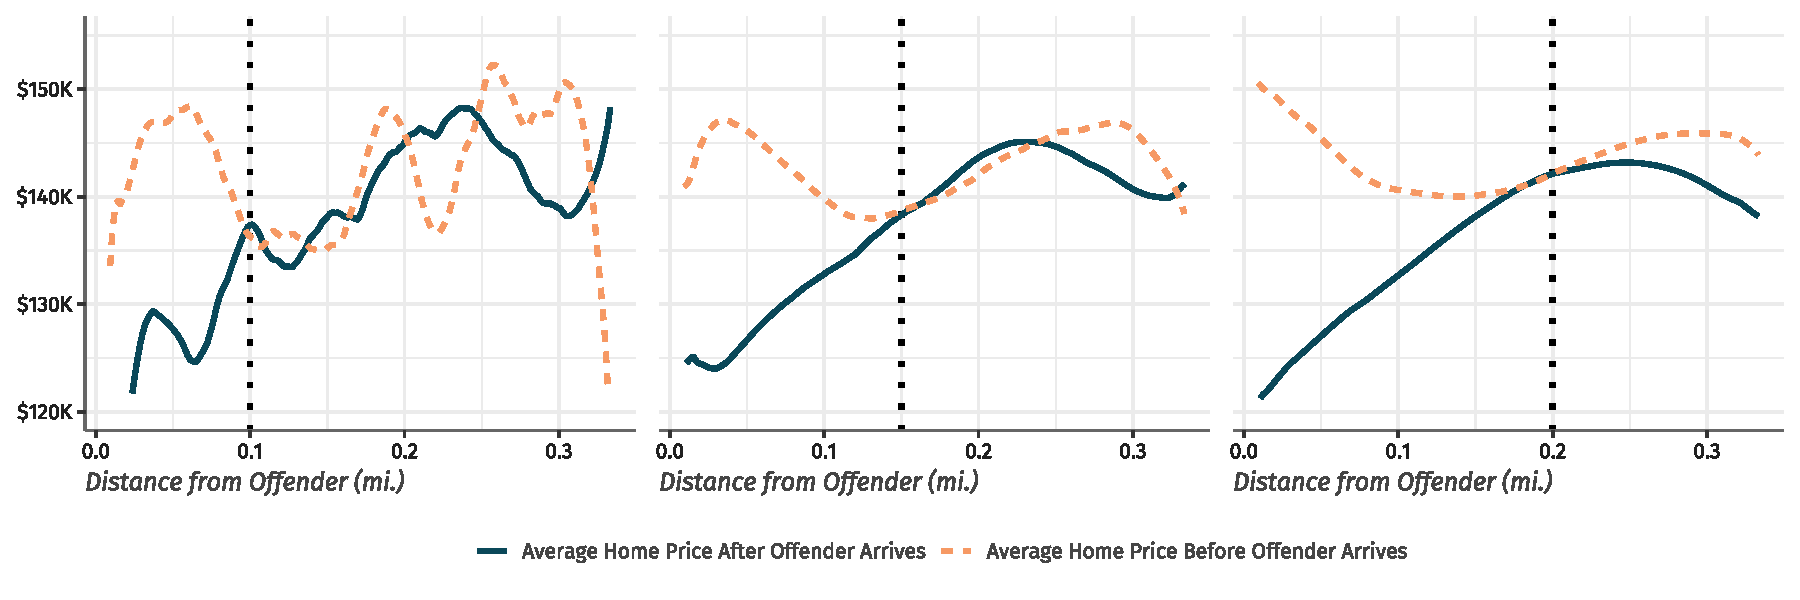
\includegraphics[width=\textwidth]{../../figures/linden_rockoff_nonparametric.pdf}
    

    {\footnotesize{\it Notes:} This figure plots estimates of home prices in the year before and the year after the arrival of a sex offender estimated using a Local Polynomial Kernel Density estimation with an Epanechnikov kernel. Panel (b) recreates Figure 2 from \citet{Linden_Rockoff_2008} and the other panels change the bandwidth.}
\end{figure}

As for the choice of the treatment ring, there is little \emph{a priori} reasons to know how far the effects of sex offender arrival will extend in the neighborhood. The authors provide graphical evidence of nonparametric estimates of the conditional mean home price at different distances in the year before and the year after the arrival of a sex offender. The published plot can be seen in Panel (b) of \autoref{fig:lr_nonparametric}. They `eyeball' the point at which the two estimates are approximately equal to decide how far treatment effects extend. However, this approach is less precise than it may seem. Panels (a) and (c) show that changing the bandwidth for the kernel density estimator will produce very different guesses at how far treatment effects extend. My proposed estimator works in a data-driven way that does not require these ad-hoc decisions.

The standard rings approach is equivalent to my proposed method with two rings: $\mathcal{D}_1$ being the treated homes between 0 and 0.1 miles away and $\mathcal{D}_2$ being the control homes between 0.1 and 0.3 miles away. The average change among $\mathcal{D}_2$ estimates the counterfactual trend and the average change among $\mathcal{D}_1$ minus the estimated counterfactual trend serves as the treatment effect. Panel (a) of \autoref{fig:lr} shows the basic results of their difference-in-differences analysis which plots estimates $\hat{\tau}_j$ for $j = 1,2$.  On average, homes between 0 and 0.1 miles decline in value by about 7.5\% after the arrival of a sex offender. \emph{As an assumption} of the rings method, homes between 0.1 and 0.3 miles away are not affected by a sex offender arrival. The choice of 0.1 miles is an untestable assumption and as seen above the evidence provided is highly dependent on the choice of bandwidth parameter. My proposed estimator does not require a specific choice for a `treated' area.

\citet{Linden_Rockoff_2008} only have access to a non-panel sample of home sales, so identification requires another assumption for identification, namely that the composition of homes at a given distance does not change over time. Further, since we can no longer form first-differences of the outcome variable, seperate nonparametric estimators must be estimated before and after treatment and subtracted from one another. Details of this theory are in the Online Appendix

\begin{figure}[tb!]
    \caption{Effects of Offender Arrival on Home Prices \citep{Linden_Rockoff_2008}}\label{fig:lr}

    \begin{subfigure}{\textwidth}
        \caption{Indicator Approach}
        \centering
        \vspace{-2.5mm}
        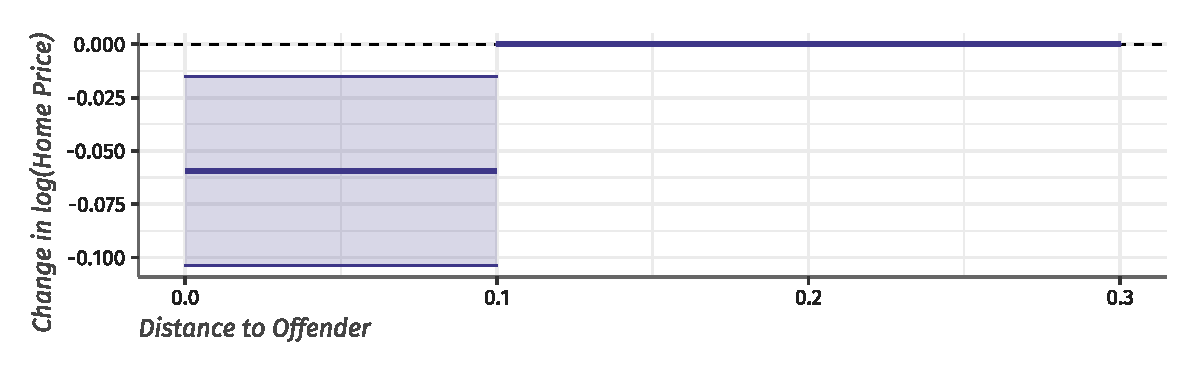
\includegraphics[width=\textwidth]{../../figures/linden_rockoff_did.pdf}
    \end{subfigure}
    \hfill
    \begin{subfigure}{\textwidth}
        \caption{Nonparametric Approach}
        \centering
        \vspace{-2.5mm}
        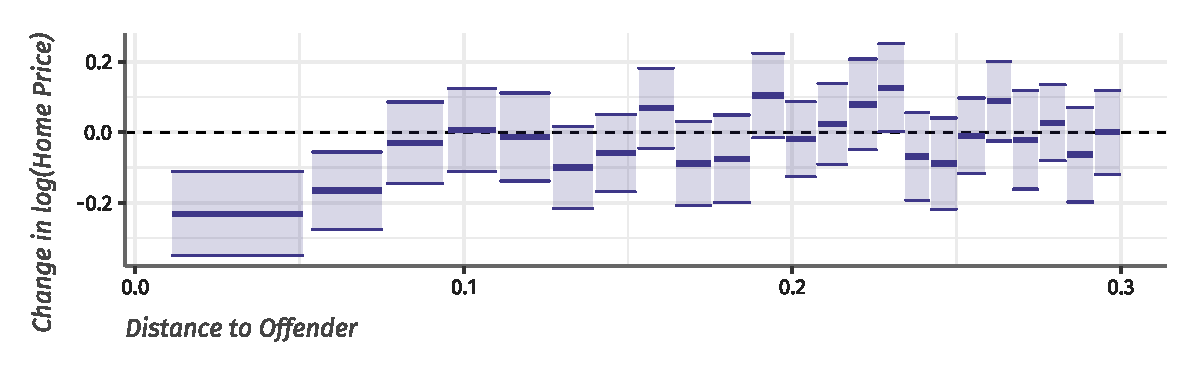
\includegraphics[width=\textwidth]{../../figures/linden_rockoff.pdf}
    \end{subfigure}

    {\footnotesize{\it Notes:} This figure plots the estimated change in home prices after the arrival of a registered sex offender as a function of distance from offender. Each line plots $\hat{\tau}_j = \overline{\Delta Y}_j - \overline{\Delta Y}_l $ with associated standard errors. Panel (a) shows an estimate from Equation \ref{eq:ring_method} with a treatment distance of $1/10^{th}$ miles and a control distance of $1/3^{rd}$ mile. Panel (b) shows the nonparametric estimate of $\tau(\dist_i)$ proposed in Section \ref{sec:lspartition}.}
\end{figure}

Panel (b) of \autoref{fig:lr} applies the nonparametric approach described in Section \ref{sec:lspartition}. Two differences in results occur. First, homes in the two closest rings i.e. within a few hundred feet, are most affected by sex-offender arrival with an estimated decline of home value of around 20\%. homes a bit further away but still within in Linden and Rockoff's `treated' sample do not experience statistically significant treatment effects. As discussed above, Linden and Rockoff's estimate of $\bar{\tau}$ is attenuated towards zero because of the inclusion of homes with little to no treatment effects, leading them to understate the effect of arrival on home prices. The nonparametric approach improves on answering this question by providing a more complete picture of the treatment effect curve. The magnitude of treatment effects decrease over distance, providing additional evidence that the arrival causes a drop in home prices.\footnote{This is similar to estimating a dose-response function as evidence supporting a causal mechanism. The results of this paper are similar to the results of \citet{Callaway_Goodman-Bacon_SantAnna_2021} with continuous treatment. In their framework, \nameref{assum:parallel} is analagous to their assumption of common trends at different doses of a continuous treatment. In this setting, I am able to provide an estimator for the treatment effect curve, the average level effect in their terminology, by relying on an assumption that the treatment effect curve $\tau(\dist)$ is homogeneous across units.} 

The second advantage of this approach is that the produced figure provides an informal test of the local parallel trends assumption. After 0.1 miles, the estimated treatment effect curve becomes centered at zero consistently. This implies that units within each ring have the same estimated trend as the outer most ring, providing suggestive evidence that homes in this neighborhood are subject to the same trends. 

% ------------------------------------------------------------------------------
\section{Conclusion}
% ------------------------------------------------------------------------------

This article formalizes a common applied identification strategy that has a strong intuitive appeal. When treatment effects of shocks are experienced in only part of an area that would otherwise be on a common neighborhood-trend, difference-in-differences comparisons within a neighborhood can identify treatment effects. However, this paper shows that the typical \emph{estimator} for treatment effects requires a very strong assumption and returns only an average treatment effect among affected units when this assumption holds. 

This article then proposes an improved estimator that relies on nonparametric series estimators. The nonparametric estimator allows for estimation of the treatment effect at different distances from treatment, similar to a dose-response function, which can allow better understanding of \emph{who} is experiencing effects and how this changes across `exposure' to a shock. More, in some cases it can provide explanation for null results. For example, if a bus station creates negative externalities for apartments that border the station but positive externalities for apartments within walking distance, the average effect could be zero. However, nonparametric estimation would reveal the two effects seperately.


% ------------------------------------------------------------------------------
\newpage~\bibliography{references.bib}
% ------------------------------------------------------------------------------

% ------------------------------------------------------------------------------
\newpage~\appendix 
% ------------------------------------------------------------------------------

% ------------------------------------------------------------------------------
\section{Proofs}
\label{sec:proofs}
% ------------------------------------------------------------------------------

% ------------------------------------------------------------------------------
\subsection{Proof of Proposition \ref{prop:ring_decomp}}
% ------------------------------------------------------------------------------

\begin{proof}
    \ Note using our model (\ref{eq:model}), we have 
    \begin{align*}
        \expec{\hat{\beta}_1} &= \condexpec{\Delta Y_{it}}{\mathcal{D}_t} - \condexpec{\Delta Y_{it}}{\mathcal{D}_c} \\
        &= \condexpec{\tau(\dist_i) + \lambda(\dist_i) + \Delta \varepsilon_{i}}{\mathcal{D}_t} - \condexpec{\tau(\dist_i) + \lambda(\dist_i) + \Delta \varepsilon_{i}}{\mathcal{D}_c} \\ 
        &= \condexpec{\tau(\dist_i)}{\mathcal{D}_t} - \condexpec{\tau(\dist_i)}{\mathcal{D}_c} + \condexpec{\lambda(\dist_i)}{\mathcal{D}_t} - \condexpec{\lambda(\dist_i)}{\mathcal{D}_c} \\ 
        &\quad + \condexpec{\Delta\varepsilon_i}{\mathcal{D}_t} - \condexpec{\Delta\varepsilon_i}{\mathcal{D}_c}.
    \end{align*}
    By construction, $\Delta \varepsilon_i$ is uncorrelated with distance, so the final two terms in the sum is zero giving us result (i). Result (ii) comes from the fact that within $d_c$, $\lambda(\dist_i) = \lambda$. Result (iii) comes from the fact that if $d_t$ is the correct cutoff $\condexpec{\tau(\dist_i)}{\mathcal{D}_c} = 0$.
\end{proof}

% ------------------------------------------------------------------------------
\subsection{Proof of Proposition \ref{prop:np_identification}}
% ------------------------------------------------------------------------------

\begin{proof}
    \ Note that $L \to \infty$ implies $d_t \leq F_n^{-1}(\frac{L-1}{L})$ by assumption (\ref{assum:dt_weak}). This implies $\overline{\Delta Y}_L \to^p \lambda$ as $n \to \infty$ by assumption (\ref{assum:dt_weak}). 
    
    From assumption (\ref{assum:parallel}) and from our model (\ref{eq:model}), we have
    \begin{align*}
        \hat{\tau}_j &= \overline{\Delta Y}_j - \overline{\Delta Y}_L \\
        &\to^p \condexpec{\tau(\dist)}{\dist \in \mathcal{D}_j} + \lambda - \lambda \\
        &= \condexpec{\tau(\dist)}{\dist \in \mathcal{D}_j}
    \end{align*}

    As $L \to \infty$ and $n \to \infty$, we have that $\mathcal{D}_j$ approaches a set containing a singular point, say $d_j$. Therefore 
    $$ 
        \hat{\tau}_j \to^p \condexpec{\tau(\dist)}{\dist = d_j}
    $$

    The sum of $\hat{\tau}_j$ therefore approach the conditional expectation function of $\tau(\dist)$ pointwisely. See \citet{Cattaneo_Farrell_Feng_2019} for proof of uniform convergence and underlying smoothness conditions for nonparametric consistency.
\end{proof}


% ------------------------------------------------------------------------------
\section{Monte Carlo Simulations} \label{sec:monte}
% ------------------------------------------------------------------------------

In the following section, I describe a set of Monte Carlo simulations that compare the standard rings method with the proposed nonparametric method. I generate a number of units on the unit circle for two periods using the following data-generating process proposed in \citet{Diamond_McQuade_2019}:
\begin{equation}\label{eq:monte}
p_{it} = 1 + \tau(\dist_i) \one_{t=1} + \beta_{\text{Lat}} \text{Lat}_i + \lambda \one_{t = 1} + \beta_{\text{Lon}} \text{Lon}_i + \varepsilon_{it},
\end{equation}
where $(\text{Lat}_i, \text{Lon}_i)$ is units' $x$ and $y$ coordinates on the unit circle, $\beta_{\text{Lat}} \sim N(0, 0.036)$ and $\beta_{\text{Lon}} \sim N(0, 0.036)$ determine how the price levels evolve over the unit circle, $\lambda \sim N(0,0.025)$ is the constant common trend, $\varepsilon_{it} \sim N(0, 0.036)$ are idiosyncratic errors (uncorrelated with distance). 

The key component of my simulations is the treatment effect curve, $\tau(\dist_i)$, which I vary across simulations:
\begin{align*}
  \tau_1(\dist) &= 0.15 * \one_{\dist < 0.4} \\
  \tau_2(\dist) &= \left( 0.5 * (0.8 - \dist)^2 \right) * 1_{\dist < 0.8} \\
  \tau_3(\dist) &= \left( -0.15 + 1.2875 * \dist - 1.375 * \dist^2 \right) * 1_{\dist < 0.8} \\
  \tau_4(\dist) &= \left( 0.5 * (0.8 - \dist)^2 \right) * 1_{\dist < 0.25} \\
\end{align*}

First, to compare the rings method and the nonparametric under favorable conditions for the ring method, I use $\tau_1$ which assumes the treatment effect curve is flat for a fixed distance which aligns with the ring method. Second, I use the treatment effect curve proposed by \citet{Diamond_McQuade_2019} which is a positive effect that declines to 0 by $\dist = 0.8$. This treatment effect curve is difficult to estimate since it evolves smoothly over space. However, the estimate of a ring might be close to the average treatment effect since the curve is positive everywhere. Third, I use $\tau_3$ which starts with a negative effect which becomes positive around $\dist = 0.3$ and then becomes 0 by $\dist = 0.8$. This treatment effect curve is the most difficult for the rings method since the average treatment effect is near zero even though there are significant positive and negative effects. Last, I modify $\tau_2$ to cuttoff at $\dist = 0.25$, so that only units \emph{really} close to treatment are affected by treatment. This is potentially difficult for the rings estimtator which will average over many non-affected units.

For each treatment effect curve, I generate data according to (\ref{eq:monte}) and estimate the treatment effect curve in three ways. I use that standard rings method with two rings $\{(0, 0.6], (0.6,1] \}$, with three rings $\{(0, 0.3], (0.3, 0.6], (0.5,1] \}$, and the nonparametric ring method proposed in section \ref{sec:lspartition}. Note that these simulations are performed with the correct maximum treatment distance satisfied, which in practice is not known. In cases where the true treatment effect distance is not known, this would introduce additional bias in the treatment effect curve estimate. 

I compare each estimator on their ability to estimate the true treatment effect curve. To do so, for each point in the data, I compute the predicted treatment effect $\hat{\tau}(\dist_i)$ and compare it to the true treatment effect $\tau(\dist_i)$. I'll label this quantity, $\upsilon_i \equiv \hat{\tau}(\dist_i) - \tau(\dist_i)$, as the prediction error. To summarize the prediction error, I calculate the mean-squared prediction error, $\hat{E}(\upsilon_i^2)$, and the average absolute prediction error, $\hat{E}( | \upsilon_i |)$, where the average is taken over the sample of observations with positive treatment effects. These numbers are a combination (i) how well the predicted treatment effect curve is approximated (bias of estimator) and (ii) the estimator's noise in repeated sampling (variance of estimator). Additonally, since it is often desirable to accurately estimate the largest treatment effects, I report the bias in predicted treatment effect at $0.4$ miles following \citet{Diamond_McQuade_2019}. For each metric, I divide by the nonparametric estimator's value, so that values $> 1$ perform worse than the nonparametric method and values $< 1$ perform better.

\begin{table}[!htbp]
  \caption{Monte Carlo Simulations} 
  \label{tab:monte}

  \begin{center}
  \begin{threeparttable}
      \begin{tabular}{@{} l @{\hskip 2.5mm} *{2}{c} @{\hskip 2.5mm} *{2}{c} @{\hskip 2.5mm} *{2}{c} @{}}
        \toprule

        & \multicolumn{2}{c}{$\hat{E}(\upsilon_i^2)$} & \multicolumn{2}{c}{$\hat{E}(|\upsilon_i|)$} & \multicolumn{2}{c}{Bias at $0.4$ miles}\\
        \cmidrule(lr){2-3} \cmidrule(lr){4-5} \cmidrule(lr){6-7} 
        
        \multicolumn{1}{l}{$n$} & \multicolumn{1}{c}{2 Rings} & \multicolumn{1}{c}{3 Rings} & \multicolumn{1}{c}{2 Rings} & \multicolumn{1}{c}{3 Rings} & \multicolumn{1}{c}{2 Rings} & \multicolumn{1}{c}{3 Rings} \\

        \toprule

        \multicolumn{7}{l}{\rule{0pt}{3mm}$\tau_1$} \\
        \midrule
        $250$  & $0.33$ & $0.46$ & $0.58$ & $0.73$ & $0.59$ & $0.87$ \\ 
$500$  & $0.26$ & $0.36$ & $0.52$ & $0.66$ & $0.54$ & $0.79$ \\ 
$1000$ & $0.21$ & $0.29$ & $0.47$ & $0.58$ & $0.49$ & $0.69$ \\ 
$5000$ & $0.12$ & $0.16$ & $0.36$ & $0.45$ & $0.38$ & $0.55$ \\ 



        \multicolumn{7}{l}{\rule{0pt}{3mm}$\tau_2$} \\
        \midrule
        $250$  & $0.81$ & $0.56$ & $1.13$ & $0.81$ & $1.68$ & $0.91$ \\ 
$500$  & $1.05$ & $0.55$ & $1.32$ & $0.84$ & $2.06$ & $1.06$ \\ 
$1000$ & $1.47$ & $0.61$ & $1.59$ & $0.93$ & $2.54$ & $1.29$ \\ 
$5000$ & $3.81$ & $1.15$ & $2.48$ & $1.32$ & $4.32$ & $2.22$ \\ 

        
        \multicolumn{7}{l}{\rule{0pt}{3mm}$\tau_3$} \\
        \midrule
        $250$  & $0.62$ & $0.72$ & $0.85$ & $0.89$ & $1.06$ & $0.98$ \\ 
$500$  & $0.72$ & $0.78$ & $0.93$ & $0.94$ & $1.21$ & $1.09$ \\ 
$1000$ & $0.91$ & $0.95$ & $1.06$ & $1.04$ & $1.45$ & $1.31$ \\ 
$5000$ & $2.18$ & $2.17$ & $1.61$ & $1.54$ & $2.49$ & $2.24$ \\ 


        \multicolumn{7}{l}{\rule{0pt}{3mm}$\tau_4$} \\
        \midrule
        $250$  & $1.57$ & $0.93$ & $1.34$ & $1.00$ & $1.37$ & $1.01$ \\ 
$500$  & $2.17$ & $1.16$ & $1.55$ & $1.14$ & $1.60$ & $1.18$ \\ 
$1000$ & $3.63$ & $1.85$ & $1.95$ & $1.44$ & $2.06$ & $1.52$ \\ 
$5000$ & $6.96$ & $3.37$ & $3.64$ & $2.67$ & $5.76$ & $4.24$ \\ 


        \bottomrule
      \end{tabular} 
      % Notes 
      \begin{tablenotes}
          \item\noindent{\footnotesize\textit{Notes.} The table shows the results from 2,000 Monte Carlo simulations. For each treatment effect curve $\tau_i$, I generate data following (\ref{eq:monte}) and estimate the treatment effect curve using the standard ring methods with 2 or 3 rings and the nonparametric method. Columns (2)-(3) report the mean-squared prediction error, (4)-(5) report the mean absolute prediction error, and (6)-(7) report the prediction error at 0.4 miles. All results are normalized by the nonparametric value, so that values $>1$ performed worse than the nonparametric method and vice-versa.}
      \end{tablenotes}
  \end{threeparttable}
  \end{center}
\end{table}

The results are presented in \autoref{tab:monte}. For $\tau_1$, the 2 ring and 3 ring method performed better than the nonparametric method across metrics and across sample sizes. This is due to (i) the large rings accurately approximate the treatment effect curve and (ii) the sampling variation of the nonparametric estimator. For $\tau_2$ and $\tau_3$, the rings estimators perform better at small sample sizes, but by 5000 observations, the nonparametric method performs better in all 3 metrics which makes sense given that nonparametric estimators perform better with larger amounts of data. Last, for $\tau_4$, the nonparametric estimator performs better than the rings method even at small sample sizes. This is because the rings method is able to better tease out the large treatment effect \emph{very close} to treatment than the rings method. Overall, the results of \autoref{tab:monte} show that the rings method performs better in most settings with at least a few thousand observations except for in the most-favorable case where the treatment effect curve is approximately flat.




\end{document}
